\ExplSyntaxOn
\sys_gset_rand_seed:n {42}
\ExplSyntaxOff
\DocumentMetadata{pdfstandard=A-3a,pdfstandard=X-5,pdfstandard=UA-1,lang=en-US,pdfversion=1.7,testphase={phase-I,firstaid,title,graphic}}

\PassOptionsToPackage{scaled=0.85}{roboto-mono}
\documentclass[
	english,
	ruledheaders=section,
	class=report,
	thesis={type=bachelor},
	accentcolor=9c,
	custommargins=true,
	marginpar=false,
	parskip=half-,
	fontsize=11pt,
    listof=totoc
]{tudapub}

\usepackage[export]{adjustbox}

\usepackage[german, main=english]{babel}

\usepackage{microtype}

\usepackage{unicode-math}

\newcommand{\todo}[2][]{{\color{red} TODO: {#2}}}

\definecolor{mygreen}{RGB}{38,162,105}

\usepackage[acronym]{glossaries-extra}

\setabbreviationstyle[acronym]{long-short}

\renewcommand{\glsxtrtitleopts}{}

\newignoredglossary{ignored}

\makeglossaries

\newglossaryentry{simple algorithm}
{
    type={ignored},
    name=simple algorithm,
    description={Our algorithm without batching and without an AVL tree}
}

\newglossaryentry{simple ID}
{
    type={ignored},
    name=simple ID,
    description={The ID for our simple algorithm}  
}

\newglossaryentry{batching ID}
{
    type={ignored},
    name=batching ID,
    description={The ID for our batching algorithm}
}

\newglossaryentry{batching algorithm}
{
    type={ignored},
    name=batching algorithm,
    description={Our algorithm with batching but without an AVL tree}
}

\newglossaryentry{simple AVL algorithm}
{
    type={ignored},
    name=simple AVL algorithm,
    description={Our algorithm without batching but with an AVL tree}
}

\newglossaryentry{batching AVL algorithm}
{
    type={ignored},
    name=batching AVL algorithm,
    description={Our algorithm with batching and with an AVL tree}
}

\newacronym{crdt}{CRDT}{conflict-free replicated data type}
\newacronym{ot}{OT}{operational transformation}
\newacronym{oo}{OO}{Object-oriented}
\newacronym{fp}{FP}{Functional programming}
\newacronym{p2p}{P2P}{peer-to-peer}
\newacronym{dtn}{DTN}{delay tolerant network}
\newacronym{rdt}{RDT}{replicated data type}
\newacronym{woot}{WOOT}{WithOut Operational Transforms}
\newacronym{rga}{RGA}{Replicated Growable Array}
\newacronym{yata}{YATA}{Yet Another Transformation Approach}
\newacronym{manet}{MANET}{mobile ad hoc network}

\usepackage{fancyvrb}
\fvset{vspace=0pt}

\usepackage[newfloat]{minted}
\setminted{linenos,frame=lines}
\usepackage{caption}
\captionsetup[listing]{skip=0pt}

\usepackage[autostyle]{csquotes}

\usepackage{biblatex}

\usepackage{cleveref}

\usepackage{subcaption}

\pdfvariable omitcidset=1

\addbibresource{literature.bib}

\makeatletter
\let\ORG@Gscale@box\Gscale@box
\long\def\Gscale@box#1{%
  \xdef\thelastscalefactor{#1}%
  \ORG@Gscale@box{#1}}
\makeatother

\ExplSyntaxOn
\makeatletter
\renewcommand*{\@author}{
    \begingroup
        \seq_use:Nnnn \g_ptxcd_author_seq {~\authorandname{}~} {,~} {~\&~}
    \endgroup
}
\makeatother
\ExplSyntaxOff

\begin{document}

\title{Optimizing Collaborative Plain~Text Editing Algorithms}
\subtitle{for Decentralized Non-Realtime Text Editing}
\author{Moritz Hedtke}
\reviewer{Prof. Dr.-Ing. Mira Mezini \and Dr.-Ing. Ragnar Mogk}

\department{inf}
\institute{TU Darmstadt}
\group{Software Technology Group}

\submissiondate{\today}
\examdate{\today}

\tuprints{urn=278347,printid=27834,year=2024}

\maketitle
\affidavit
\begin{abstract}[english]
    Text editing is ubiquitous, as it occurs on almost every website, mobile app, and desktop application. Collaborative text editing avoids manual synchronization when working together with others on text. This requires algorithms that can efficiently combine the concurrent edit operations in an intent-preserving way. Additionally, supporting a wide range of network scenarios enables offline work in a decentralized manner with better availability and reliability than with central servers. In this thesis, we first look at prior solutions for plain text editing and their ability to preserve user intentions, as users should not experience unexpected behavior when concurrently editing text. Then, we improve the benchmarking approach of prior research to estimate asymptotic complexity and to measure performance of algorithmic edge cases. Based on that, we propose optimizations for a prior collaborative text editing algorithm called Fugue. Our optimized algorithm can handle character insertion and deletion in logarithmic runtime in relation to the text length and with constant memory usage per character operation. It uses 25 bytes and one microsecond per operation on four Intel Xeon Gold vCPUs for a representative text with 25 million operations. We also develop a local web application as a proof of concept for working on plain text collaboratively using WebRTC. Additionally, we show that the maximally non-interleaving property in the Fugue paper can exhibit interleaving when deletions are involved.
\end{abstract}
\tableofcontents

\newlength{\imagea}
\newlength{\imageb}

\newcommand{\twoMinipageFigures}[4]{
    \settoheight{\imagea}{\includegraphics{#1}}
    \settoheight{\imageb}{\includegraphics{#3}}

    \ifdim\imagea>\imageb
        \begin{figure}
            \begin{minipage}[t]{.4875\textwidth}
                \sbox0{\includegraphics[max width=\textwidth,valign=t]{#1}}
                \includegraphics[scale=\thelastscalefactor,valign=t]{#1}
                #2
            \end{minipage}
            \hfill
            \begin{minipage}[t]{.4875\textwidth}
                \includegraphics[scale=\thelastscalefactor,valign=t]{#3}
                \vphantom{\includegraphics[scale=\thelastscalefactor,valign=t]{#1}}
                #4
            \end{minipage}
        \end{figure}
    \else
        \begin{figure}
            \begin{minipage}[t]{.4875\textwidth}
                \sbox0{\includegraphics[max width=\textwidth,valign=t]{#3}}
                \includegraphics[scale=\thelastscalefactor,valign=t]{#1}
                \vphantom{\includegraphics[scale=\thelastscalefactor,valign=t]{#3}}
                #2
            \end{minipage}
            \hfill
            \begin{minipage}[t]{.4875\textwidth}
                \includegraphics[scale=\thelastscalefactor,valign=t]{#3}
                #4
            \end{minipage}
        \end{figure}
    \fi
}

\newcommand{\twoSubfigures}[4]{
    \settoheight{\imagea}{\includegraphics{#1}}
    \settoheight{\imageb}{\includegraphics{#3}}

    \ifdim\imagea>\imageb
        \begin{subfigure}{.5\textwidth}
            \sbox0{\includegraphics[max width=\textwidth,valign=t]{#1}}
            \includegraphics[scale=\thelastscalefactor,valign=t]{#1}
            #2
        \end{subfigure}%
        \begin{subfigure}{.5\textwidth}
            \includegraphics[scale=\thelastscalefactor,valign=t]{#3}
            \vphantom{\includegraphics[scale=\thelastscalefactor,valign=t]{#1}}
            #4
        \end{subfigure}%
    \else
        \begin{subfigure}{.5\textwidth}
            \sbox0{\includegraphics[max width=\textwidth,valign=t]{#3}}
            \includegraphics[scale=\thelastscalefactor,valign=t]{#1}
            \vphantom{\includegraphics[scale=\thelastscalefactor,valign=t]{#3}}
            #2
        \end{subfigure}%
        \begin{subfigure}{.5\textwidth}
            \includegraphics[scale=\thelastscalefactor,valign=t]{#3}
            #4
        \end{subfigure}%
    \fi
}

\newcommand{\benchmarkResults}[2]{
    \begin{figure}
        \begin{subfigure}{.5\textwidth}
            \includegraphics[width=\textwidth]{../text-rdt/jvm/figure-benchmark-results/#1.pdf}
            \caption{time}
            \label{fig:#1-time}
        \end{subfigure}%
        \begin{subfigure}{.5\textwidth}
            \includegraphics[width=\textwidth]{../text-rdt/jvm/figure-benchmark-results/#1-memory.pdf}
            \caption{memory}
            \label{fig:#1-memory}
        \end{subfigure}
        \caption{#2}
        \label{fig:#1}
    \end{figure}
}

\newcommand{\evilEdgeCase}[2]{
    \begin{figure}
        \twoSubfigures{../text-rdt/target/pdfs/#1-before.pdf}{\caption{before}
            \label{fig:edge-case-#1-before}}{../text-rdt/target/pdfs/#1-after.pdf}{\caption{after}
            \label{fig:edge-case-#1-after}}
        \caption{Example for #2}
        \label{fig:edge-case-#1-example}
    \end{figure}
}

\IMRADlabel{introduction}
\chapter{Introduction} \label{introduction}

Nearly all applications require text editing in some form --- even if just for text entry into a form element. When we want to make these applications collaborative, those text fields need collaborative text editing. However, such functionality is not yet easily available. In contrast to single user text editing, collaborative text editing creates challenges with merging concurrent edit operations and especially handling conflicting edit operations and performance edge cases. Collaborative text editing algorithms need to handle conflicts in an intent-preserving and converging way.

Prior collaborative solutions require a central server, such as Microsoft~365 and Google Docs, or open source variants such as MediaWiki (which powers Wikipedia), Overleaf, Etherpad, Collabora Online or OnlyOffice. Needing a central server for text editing can be undesired for several reasons. First, when the server is operated by a third party it usually requires sending the text to the third party to handle the edit actions. Second, this creates a dependency on the availability of the server. The availability can be affected by power outages, cyberattacks, software and hardware failures including the network, overloading or natural disasters. Third, this also creates a dependency on the reliability or integrity of the server. Software and hardware failures especially of the storage can destroy the data, cyberattacks and human mistakes can manipulate or destroy the data, natural disasters or fire can destroy the server. Examples for such issues are OVHcloud's burned down data center, CrowdStrike, the Facebook BGP outage, the Google Cloud UniSuper incident, the XZ Utils backdoor, WannaCry, and many others.

Similarly, the client may not be able to reach the server. This may be the case when public infrastructure like cell towers is unavailable, because of natural disasters, sabotage, cyberattacks, failure of infrastructure they depend on such as the power grid or for any other reason. A recent example are the Ahrtal floods.

Decentralized algorithms can adapt to these challenges by functioning in a wide range of network scenarios. For example, \gls{p2p} networks work without a central server. Furthermore, \glspl{manet} and \glspl{dtn} do not require public communication infrastructure at all but instead can utilize Wi-Fi, Bluetooth and other short-range communication technology.

In a decentralized setting there is no guarantee that peers are frequently online. Therefore, the ability to handle \textit{non-realtime} editing with potentially long periods of offline activity is essential. This combination of offline and decentralized software is often called local-first software \cite{2019-kleppmann-local-first}.

The two major ways in research to approach collaborative text editing are \gls{ot} and \glspl{crdt} \cite[page 2]{2019-sun-difference-ot-crdt-1-general-transformation-framework}. \gls{ot} algorithms store edit operations based on the text position and therefore need to transform concurrent edit operations against each other to correct the text positions. Then, the algorithms apply the operations directly to the text.
Prior algorithms for \gls{ot} are, for example, COT \cite{2009-sun-ot-context-undo} and Jupiter \cite{1995-nichols-jupiter}. While some of these are \textit{not} able to work in a decentralized network but need a central server to order changes like Jupiter \cite{1995-nichols-jupiter}, a lot of them \textit{are} able to work in a decentralized network like COT \cite{2009-sun-ot-context-undo} \cite[Section 4]{2019-sun-difference-ot-crdt-3-building-real-world-applications}. Prior \gls{ot} algorithms have a runtime complexity per remote operation that is linear in the amount of concurrent edit operations \cite[Section 3.1.4]{2019-sun-difference-ot-crdt-2-correctness-complexity}. This makes them really efficient for \textit{near-realtime} editing where only few concurrent edit operations occur. Near-realtime editing means that only short connection interruptions happen \cite{2016-yata-yjs}. For \textit{non-realtime} text editing this leads to a highly inefficient runtime complexity because the many concurrent edit operations must be transformed against each other \cite[Section 1]{2019-sun-difference-ot-crdt-3-building-real-world-applications}. Therefore, prior \gls{ot} algorithms are undesirable for supporting a wide range of network scenarios like \glspl{dtn}.

In contrast, \glspl{crdt} associate parts of the text with identifiers and merge these together on synchronization. Therefore, they need to convert between identifiers and text positions to handle text edit operations. Prior algorithms for \glspl{crdt} are, for example, \gls{woot} \cite{2006-oster-woot}, Logoot \cite{2009-weiss-logoot}, \glspl{rga} \cite{2011-roh-rga} and Fugue \cite{2023-weidner-minimizing-interleaving}. \glspl{crdt} work in decentralized networks, but each prior algorithm has shortcomings that make it undesirable for a general solution. For example, Logoot \cite{2009-weiss-logoot} has quadratic memory use in some cases. Also, for handling text of some length their runtime complexity is often quadratic or worse in relation to the text length, as with \gls{woot} \cite{2006-oster-woot}, \gls{rga} \cite{2011-roh-rga} and Fugue \cite{2023-weidner-minimizing-interleaving} \cite[Section 5.3]{2019-sun-difference-ot-crdt-1-general-transformation-framework}.

While Fugue \cite{2023-weidner-minimizing-interleaving} avoids interleaving issues of prior solutions and works in an offline setting, the current implementation for handling text of some length has quadratic runtime complexity in relation to the text length.

In this thesis, we first investigate suitable algorithms for local-first plain text editing to integrate into our Scala based applications, see \Cref{chapter:challenges}. Based on the evaluation of prior solutions in Fugue \cite{2023-weidner-minimizing-interleaving}, we consider interleaving the major issue apart from performance issues, see \Cref{section:challenges-text-interleaving}. Therefore, we extensively investigate how the Fugue algorithm avoids interleaving by looking at the algorithm, the examples and the proofs in the Fugue paper \cite{2023-weidner-minimizing-interleaving}, see \Cref{section:challenges-text-interleaving-fugue}. Additionally, we show that the property of \textit{maximally non-interleaving} in the Fugue paper \cite{2023-weidner-minimizing-interleaving} still allows interleaving when deletions are involved.
\Cref{chapter:ot} gives an insight into \glspl{crdt} and \gls{ot} and their advantages and disadvantages.

Then, \Cref{chapter:background} describes the Fugue algorithm \cite{2023-weidner-minimizing-interleaving} in depth.
\Cref{section:implementation} discusses our base implementation of Fugue in Scala to be able to experiment with the algorithm and proposes using property tests to ensure the convergence of our implementation. For easier experimentation and as a showcase we create a local web application to collaboratively edit a text using WebRTC.

The benchmarks in \Cref{optimization} show that the base implementation has severe performance issues. Therefore, we optimize our implementation based on our benchmarks and propose optimizations of the Fugue algorithm. Through the use of binary search trees at relevant places with some use-case specific customizations we achieve amortized logarithmic runtime per character insertion or deletion and thus an amortized runtime of $O(n \log(n))$ for handling $n$ character operations. Additionally, we implement batching of sequential insertions to reduce memory usage, which was already roughly mentioned in the Fugue paper without details on the exact implementation \cite{2023-weidner-minimizing-interleaving}. Furthermore, we contribute a benchmark that in comparison to prior work shows the asymptotic runtime and focuses on edge cases in the algorithm that may have performance characteristics different from those of the common execution path. Specifically, we focus on ensuring that the algorithm also has an acceptable runtime complexity when considering malicious or unexpected behavior of peers.

We evaluate our optimized implementation in \Cref{chapter:evaluation} and show that we achieve the targeted $O(n \log(n))$ runtime complexity with a runtime of one microsecond per character operation and memory use of 25 bytes per operation for a realistic editing session on four Intel Xeon Gold vCPU.
Finally, \Cref{chapter:future-work} shows future work such as rich text editing, and \Cref{chapter:conclusion} concludes our work.

\chapter{Challenges with Collaborative Text Editing} \label{chapter:challenges}

This chapter first introduces the goal of user intent-preservation by showing the problem of text interleaving in \Cref{section:challenges-text-interleaving}. Then, \Cref{section:challenges-text-interleaving-fugue} introduces the solution proposed by Fugue \cite{2023-weidner-minimizing-interleaving} to solve text interleaving. Finally, \Cref{chapter:ot} compares \glspl{crdt} and \gls{ot} and shows that the current \glspl{crdt} runtime complexity is quadratic and current \gls{ot} algorithms are unsuitable for \textit{non-realtime} editing.

\section{Text Interleaving} \label{section:challenges-text-interleaving}

When users write text in a collaborative text editor, they expect that their text is not modified in an unexpected way by concurrent edits from other users. One example are insertions at \textit{different} positions. Starting with the text \texttt{"Alice plays Minecraft"}, \textcolor{red}{Alice} changes the text to \texttt{"Alice \textcolor{red}{happily} plays Minecraft"}. Concurrently, \textcolor{blue}{Bob} changes the text to \texttt{"Alice plays Minecraft \textcolor{blue}{with Bob}"}. Then, the expected result after synchronizing is \texttt{"Alice \textcolor{red}{happily} plays Minecraft \textcolor{blue}{with Bob}"}. As the insertions are at different positions in the text, the expected outcome is unambiguous, and all characters should stay at their relative position to the surrounding characters.
Users also expect that text they wrote in one go is not interleaved by text that another user wrote concurrently. An example with insertions at the \textit{same} position is the following. Starting with the text \texttt{"milk, chocolate"}, \textcolor{red}{Alice} changes the text to \texttt{"milk, \textcolor{red}{eggs,} chocolate"} and \textcolor{blue}{Bob} concurrently changes the text to \texttt{"milk, \textcolor{blue}{bread,} chocolate"}. The expected result after synchronizing is either \texttt{"milk, \textcolor{red}{eggs,} \textcolor{blue}{bread,} chocolate"} or \texttt{"milk, \textcolor{blue}{bread,} \textcolor{red}{eggs,} chocolate"}. While there are two possibilities in this case, no interleaving occurs in either case.

\begin{figure}
  \centering
  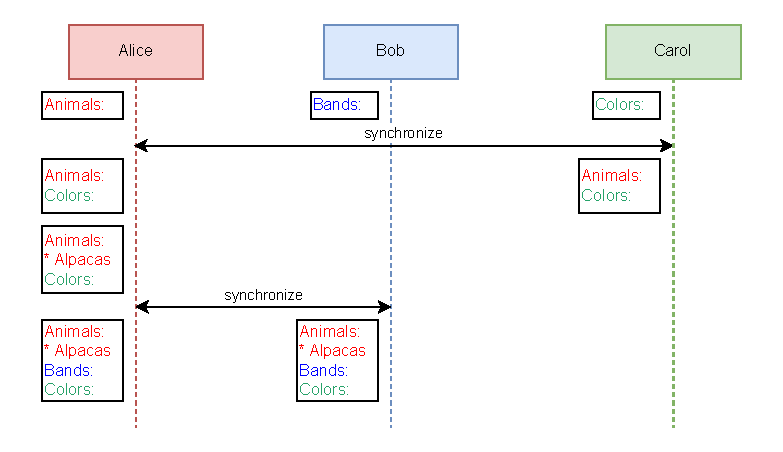
\includegraphics[width=\textwidth]{figures/forward-more-important-than-backward.drawio.pdf}
  \caption{Example for prioritizing forward insertions inspired by Figure 6 in Fugue \protect\cite{2023-weidner-minimizing-interleaving}}
  \label{fig:forward-more-important-than-backward}
\end{figure}

\clearpage

For an insertion in the middle of a text, current editing behavior does not convey whether the insertion semantically belongs to the left side or the right side. Because most text is written in a forward direction, so for left-to-right script from left to right, it is more likely that an insertion in the middle of some text is appending to the left side of the insertion point instead of prepending to the right side of the insertion point. \Cref{fig:forward-more-important-than-backward} exemplifies this. The three replicas \textcolor{red}{Alice}, \textcolor{blue}{Bob} and \textcolor{mygreen}{Carol} independently add three lists to some text. Then, \textcolor{red}{Alice} and \textcolor{mygreen}{Carol} synchronize. Afterwards, \textcolor{red}{Alice} adds \texttt{"\textcolor{red}{*~Alpacas}"} to her list, such that it comes after \texttt{"\textcolor{red}{Animals:}"} and before \texttt{"\textcolor{mygreen}{Colors:}"} but inherently there is no information to which part it belongs. Finally, \textcolor{red}{Alice} and \textcolor{blue}{Bob} synchronize. This separates \texttt{"\textcolor{red}{*~Alpacas}"} and \texttt{"\textcolor{mygreen}{Colors:}"} by the received \texttt{"\textcolor{blue}{Bands:}"}, which may not be wanted. In this example the assumption of the more common forward insertion is correct though. Further improvements to this would need analysis of the language semantics of the text which \Citeauthor*{2023-bauwens-nlp-for-merging} looked into \cite{2023-bauwens-nlp-for-merging}. For the concrete example, a different idea could be to insert \texttt{"\textcolor{blue}{Bands:}"} after \texttt{"\textcolor{mygreen}{Colors:}"} so \texttt{"\textcolor{red}{*~Alpacas}"} stays in place in relation to the text preceding and following it. Unfortunately this would lead to even more unexpected behavior for example when \textcolor{blue}{Bob} and \textcolor{mygreen}{Carol} synchronized before and would order the entries alphabetically because they do not know about the insertion of \texttt{"\textcolor{red}{*~Alpacas}"}. As soon as \textcolor{red}{Alice} would then synchronize with them, the entries would need to be reordered, so that they converge. As the synchronized data is not structured like the example may suggest, but instead consists of arbitrary characters, this reordering could result in sentence reordering or other unwanted results. Another idea could be to prefer the side by the same replica. This has similar issues if concurrent edits are received later and change the effect of that rule.

\section{Fugues Approach to Avoid Text Interleaving} \label{section:challenges-text-interleaving-fugue}

This section shows the proposed solution by Fugue \cite{2023-weidner-minimizing-interleaving} to solve text interleaving. It also gives an example that the proposed \textit{maximally non-interleaving} property can still interleave text when deletions are involved.

\Citeauthor*{2023-weidner-minimizing-interleaving} \cite{2023-weidner-minimizing-interleaving} show that a previous attempt at formalizing a property for non-interleaving by \Citeauthor*{2019-Kleppmann-incorrect-noninterleaving-property} \cite{2019-Kleppmann-incorrect-noninterleaving-property} is incorrect \cite[Section 2.5]{2023-weidner-minimizing-interleaving}. Therefore, they propose their own property which they refer to as \textit{maximally non-interleaving}. It associates every inserted character with the character to its left and right, which they label left and right origin. The property orders the characters by prioritizing keeping the left origin as the previous character because of the common forward insertions and otherwise ordering to preserve the right origin as the following character if possible. Only if both origins are the same, the order is arbitrary but deterministically chosen. Therefore, this property creates a unique order aside from tie-breaking \cite[Section 4.5]{2023-weidner-minimizing-interleaving}.

Fugue refers to an interleaving issue as forward interleaving, when only one character has another character as a left origin, yet the two characters are not consecutive. One example where the Logoot algorithm \cite{2009-weiss-logoot} interleaved characters, which also violates this rule, is concurrently inserting \texttt{"\textcolor{blue}{bread}"} and \texttt{"\textcolor{red}{eggs}"}, producing \texttt{"\textcolor{blue}{b}\textcolor{red}{e}\textcolor{blue}{r}\textcolor{red}{g}\textcolor{blue}{e}\textcolor{red}{g}\textcolor{blue}{a}\textcolor{red}{s}\textcolor{blue}{d}"} \cite[Section 4.4.1]{2019-sun-difference-ot-crdt-2-correctness-complexity}. For example the \texttt{"\textcolor{blue}{r}"} from \texttt{"\textcolor{blue}{bread}"} has the \texttt{"\textcolor{blue}{b}"} as its left origin and no other character has the \texttt{"\textcolor{blue}{b}"} as its left origin but in the result they are not consecutive characters.

\Citeauthor*{2023-weidner-minimizing-interleaving} refer to another problem that many prior algorithms exhibit as backward interleaving. When two insertions have the same left origin but a different right origin, they should be ordered in a way that they are consecutive with their right origins. Although it may seem this is not a common use case, the following is a plausible example \cite[Figure 2]{2023-weidner-minimizing-interleaving}. Starting with the text \texttt{"Shopping"}, \textcolor{red}{Alice} first appends \texttt{"\textcolor{red}{*~apples}"} after \texttt{"Shopping"} and then prepends \texttt{"\textcolor{red}{Fruit:}"} before \texttt{"\textcolor{red}{*~apples}"}. While semantically she is prepending, both inserted texts have \texttt{"Shopping"} as their left origin and different right origins. Concurrently, \textcolor{blue}{Bob} first appends \texttt{"\textcolor{blue}{*~bread}"} after \texttt{"Shopping"} and then prepends \texttt{"\textcolor{blue}{Bakery:}"} before \texttt{"\textcolor{blue}{*~bread}"}. The category insertions by \textcolor{red}{Alice} and \textcolor{blue}{Bob} both have \texttt{"Shopping"} as their left origin but different right origins. Therefore, this should lead to either the outcome of \texttt{"Shopping\textcolor{red}{Fruit:*~apples}\textcolor{blue}{Bakery:*~bread}"} or \texttt{"Shopping\textcolor{blue}{Bakery:*~bread}\textcolor{red}{Fruit:*~apples}"} which only differ in the order of which users text comes first, which is arbitrary. When algorithms exhibit backward interleaving, \texttt{"Shopping\textcolor{blue}{Bakery:}\textcolor{red}{Fruit:}\textcolor{blue}{*~bread}\textcolor{red}{*~apples}"} can be a possible result.
Note that the order of the elements has not changed in relation to each other (e.g. \texttt{"\textcolor{red}{Fruit:}"} comes before \texttt{"\textcolor{red}{*~apples}"} and after \texttt{"Shopping"}) but this still violates the intent of the user.

According to \Citeauthor*{2023-weidner-minimizing-interleaving}, many popular algorithms they looked into exhibit either forward or backward interleaving \cite[Table 1]{2023-weidner-minimizing-interleaving}. A review by \Citeauthor*{2023-sun-critical-examination-fugue-ot} \cite{2023-sun-critical-examination-fugue-ot,2023-sun-critical-examination-fugue-ot-1,2023-sun-critical-examination-fugue-ot-2,2023-sun-critical-examination-fugue-ot-3} that refutes these claims for OT algorithms is addressed in \Cref{chapter:ot}. For Logoot \cite{2009-weiss-logoot} the character-by-character interleaving issue occurs. Further examples are provided in the appendix of the Fugue paper \cite{2023-weidner-minimizing-interleaving}. While the prior \gls{crdt} algorithms YjsMod\footnote{\url{https://github.com/josephg/reference-crdts}} and Sync9\footnote{\url{https://braid.org/sync9}} do not exhibit interleaving \cite[Table 1]{2023-weidner-minimizing-interleaving}, those approaches were not considered here due to the lack of documentation and their intrinsic complexity. \Citeauthor*{2023-weidner-minimizing-interleaving} propose their own algorithms Fugue and FugueMax to solve these problems. They conjecture that Sync9 is semantically equivalent to Fugue and YjsMod is semantically equivalent to FugueMax \cite[Section 6]{2023-weidner-minimizing-interleaving}. They also prove that FugueMax fulfills the \textit{maximally non-interleaving} property \cite[Theorem 9]{2023-weidner-minimizing-interleaving}, prove that the Fugue algorithm is always forward non-interleaving \cite[Lemma 7]{2023-weidner-minimizing-interleaving} and argue that it is also backward non-interleaving when there are not multiple interacting concurrent updates \cite[Section 4.3]{2023-weidner-minimizing-interleaving}.

A counter example that interleaving can also happen for the \textit{maximally non-interleaving} FugueMax algorithm is the following. Starting with the text \texttt{"Shopping"}, \textcolor{red}{Alice} appends \texttt{"\textcolor{red}{*~apples}"} after \texttt{"Shopping"} and then prepends \texttt{"\textcolor{red}{Fruit:}"} before \texttt{"\textcolor{red}{*~apples}"}. Concurrently, \textcolor{blue}{Bob} appends \texttt{"\textcolor{blue}{*~bread}"} after \texttt{"Shopping"}, then deletes and reinserts the \texttt{"\textcolor{blue}{g}"} of \texttt{"Shopping"} and finally prepends \texttt{"\textcolor{blue}{Bakery:}"} before \texttt{"\textcolor{blue}{*~bread}"}. The expected result would be \texttt{"Shoppin\textcolor{blue}{gBakery:*~bread}\textcolor{red}{Fruit:*~apples}"} but the actual result can be \texttt{"Shoppin\textcolor{blue}{gBakery:}\textcolor{red}{Fruit:*~apples}\textcolor{blue}{*~bread}"} when the replicas IDs have a specific order. The code in \Cref{appendix:code-fuguemax-interleaving} verifies this with the reference implementation\footnote{\url{https://github.com/mweidner037/fugue}}. The reason the \textit{maximally non-interleaving} property does not cover this case is that it disregards deletions. This example shows that this simplification is not suitable to ensure non-interleaving.

The basic implementation of Fugue has a linear runtime per character insertion or deletion in relation to the text length (including deleted text) which proved to be too inefficient for larger text given the resulting runtime scales quadratically with the text length. Comparing the results\footnote{\url{https://github.com/mweidner037/fugue/blob/main/results_table.md}} from \Citeauthor*{2023-weidner-minimizing-interleaving} for benchmark B1.1 with benchmark B1.3 indicates, that even the optimized variant in the Fugue paper has quadratic runtime for sequential backward insertions.

\clearpage

\begin{figure}
  \centering
  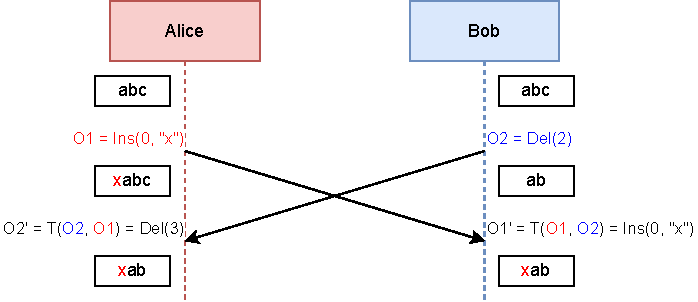
\includegraphics[width=\textwidth]{figures/ot.drawio.pdf}
  \caption{Example for operation transformation with two synchronizing peers based on figure by \Citeauthor*{2024-sun-ot-faq} \cite[Section 1.4 Figure 1]{2024-sun-ot-faq}}
  \label{fig:ot-example}
\end{figure}

\begin{listing}
  \begin{minted}{text}
Tii(Ins[p1,c1], Ins[p2, c2]) {
  if p1 < p2 or (p1 = p2 and u1 > u2)
    return Ins[p1, c1];              
  else
    return Ins[p1+1, c1];
}
\end{minted}
  \caption{Example for transformation function from Sun \cite[Section 2.15]{2024-sun-ot-faq}}
  \label{lst:example-transformation-function}
\end{listing}

\clearpage

\section{OT in Comparison to CRDTs} \label{chapter:ot}

This section explains the differences and similarities between \gls{ot} and \glspl{crdt} and shows that the current \glspl{crdt} runtime complexity is quadratic and current \gls{ot} algorithms are unsuitable for \textit{non-realtime} editing.

While \gls{crdt} papers often claim \glspl{crdt} are superior to \gls{ot}, \glspl{crdt} often miss major relevant parts of the required algorithmic steps which makes them seem potentially simpler and more performant \cite[page 2]{2019-sun-difference-ot-crdt-1-general-transformation-framework}. For example, \glspl{crdt} need to extract the text from their internal state and need to be able to address characters based on their text position as most text editors work that way \cite[Section 5.1, Section 5.2]{2019-sun-difference-ot-crdt-1-general-transformation-framework}. \Glspl{crdt} often miss this conversion step which is a major algorithmic complication that also affects their performance a lot \cite[page 2]{2019-sun-difference-ot-crdt-1-general-transformation-framework}. Note that Fugue also has this issue as it does not describe converting the received operations to character offsets \cite[Algorithm 1]{2023-weidner-minimizing-interleaving}.

\Citeauthor*{2019-sun-difference-ot-crdt-1-general-transformation-framework} also show that both approaches are more similar than often presented \cite[Section 4.1 Table 1]{2019-sun-difference-ot-crdt-1-general-transformation-framework}. While \glspl{ot} have position based operations directly on the character sequence that are then transformed by concurrent operations, \glspl{crdt} have identifier based operations on an internal object sequence, that are converted to the position based character sequence after the operations have been applied.

\gls{ot} based algorithms consist of a control algorithm and a transformation function \cite{2024-sun-ot-faq}. The control algorithm is generic, and the transformation function is application specific. For example for plain text editing there could be two operations, Insert(index, character) and Delete(index). The transformation function $T(O_2, O_1)$ transforms $O_2$ against $O_1$. This produces the operation that needs to be applied after $O_1$ if they were concurrent before. \Cref{fig:ot-example} shows an example where the positions of the concurrent operations are transformed when receiving them and therefore result in the same text at both peers. In that example the transformation function could be defined as shown in \Cref{lst:example-transformation-function} for transforming two insert operations \cite[Section 2.15]{2024-sun-ot-faq}. If a concurrent insertion happened at a position after the current insertion it does not need to be transformed. If a concurrent insertion happened at a position before the current insertion it needs to be offset by one. For equal positions, tie breaking using the replica identifier is required.

The control algorithms decide in which order operations need to be transformed to achieve the desired outcome \cite[Section 2.2]{2024-sun-ot-faq}. Depending on the control algorithm, the transformation function needs to fulfill different properties to ensure correctness \cite[Section 2.20]{2024-sun-ot-faq}. Also, some control algorithms are able to handle undo, some can undo arbitrary actions out of order, while some cannot \cite[Section 2.12]{2024-sun-ot-faq}.

Transformation functions need to be defined for all possible combinations of operations. This means $N^2$ such functions are needed for $N$ possible operations. An alternative proposed by \Citeauthor*{2019-sun-difference-ot-crdt-3-building-real-world-applications} is POT+COA (Primitive Operation
Transformation plus Complex Operation Adaptation). It consists of having some primitive operations for which transformation functions are defined, and then complex application operations are converted to these primitive operations \cite[Section 2.1.3]{2019-sun-difference-ot-crdt-3-building-real-world-applications}.

OT based algorithms can be integrated into existing editors with little change of the editors source code as OT is operation and concurrency-centric. The algorithm can just apply the received and transformed operations to the local editor and send local operations to other peers. \Citeauthor*{2019-sun-difference-ot-crdt-3-building-real-world-applications} refer to this as Transparent Adaptation (TA) \cite[Section 2.1.2]{2019-sun-difference-ot-crdt-3-building-real-world-applications}.

According to \Citeauthor*{2019-sun-difference-ot-crdt-1-general-transformation-framework}, \gls{ot} uses a concurrency-centric and direct transformation approach and \gls{crdt} uses a content-centric and indirect transformation approach \cite[Section 1]{2019-sun-difference-ot-crdt-1-general-transformation-framework}. This has an important consequence for the time and space complexity. The time and space complexity of \gls{ot} for \textit{realtime} editing depends on the number of concurrent operations which are usually small in realtime text editing while the time and space complexity of \gls{crdt} depends on the length of the text or even the length of the text including all deleted content which are usually a lot larger \cite[Section 5.3]{2019-sun-difference-ot-crdt-1-general-transformation-framework}. The time complexity for prior \gls{ot} based algorithms is at least $O(c)$ per remote operation \cite[Section 3.1.4]{2019-sun-difference-ot-crdt-2-correctness-complexity}. This means quadratic runtime complexity in relation to the operation count for handling some count of operations, which is unusable for \textit{non-realtime} editing because there can be many concurrent operations. It is important to mention that the time complexity class is relevant. For example, $O(\log(\text{text-length-including-deletions}))$ runtime complexity can be equally acceptable to $O(\text{concurrent-operations})$ runtime complexity because $O(\log(n))$ is growing quite slowly even for extremely large inputs. Prior research of \glspl{crdt} mostly managed a linear time complexity or worse except of a paper by \Citeauthor*{2016-briot-logn-optimization} which optimizes an \gls{rga} adaptation to $O(\log(n))$ per operation similarly to us \cite[Table 4]{2019-sun-difference-ot-crdt-2-correctness-complexity}. However, \Citeauthor*{2016-briot-logn-optimization} have not gone into the analysis of performance edge cases prohibiting us from drawing a fair comparison. Additionally, it is unclear whether they include the conversion of remote operations to character positions. Furthermore, as the algorithm is based on \gls{rga}, it exhibits interleaving \cite[Table 1]{2023-weidner-minimizing-interleaving}.

While \glspl{crdt} often seem to be simple and easy to understand, the fundamental concurrency issues which are inherent to unconstrained co-editing also exist there and mixing content and concurrency creates new difficulties with handling them \cite[Section~4]{2019-sun-difference-ot-crdt-2-correctness-complexity}.

\chapter{Fugue Algorithm} \label{chapter:background}

This chapter explains how the Fugue algorithm works and is heavily based on the Fugue paper \cite{2023-weidner-minimizing-interleaving}. Then, the next chapter discusses our implementation of Fugue. Further chapters discuss our improvements to the Fugue algorithm. The Fugue algorithm handles insertions and deletions for a list data structure and avoids interleaving. For text editing every list element is a character.

\section{Traversal}

\Cref{fig:fugue-traversal} visualizes the data structure of the algorithm. It is a tree starting with the root node at the top left. The nodes are connected using lines. Lines downwards to the right connect to a right child and lines downwards to the left connect to a left child. A node can have multiple children on each side. For every node except the root node, the first part is the character or whether the character is deleted, followed by a space and the ID of the peer that created that character, a \texttt{\#} symbol and then a counter for that peer that is increasing for every insertion. For example, \texttt{"t A\#1"} is the character \texttt{"t"} by peer \texttt{"A"} with the counter being $1$. The ID of the peer combined with the counter that uniquely identifies an element is called a \gls{simple ID}. The root node is a special node that behaves like a deleted character. To get the current text of the tree, it is traversed starting from the root node by recursively visiting the left children in order, then the value of the node itself and then the right children in order. For the example in \Cref{fig:fugue-traversal}, the traversal starts with the left children of the root node. As there are none, the node itself is visited. As it contains a deleted character, it is ignored. Then the first right child is traversed. Its first left child produces \texttt{"small~"} by the same rules applied recursively. It itself produces \texttt{"t"}. Its right children produces \texttt{"rees"}. Therefore, its whole traversal produces \texttt{"small~trees"}. Then the second right child is traversed in the same way and produces \texttt{"~grow"}. Combining all that will therefore produce the text \texttt{"small~trees~grow"}.

\clearpage

\begin{figure}
  \includegraphics[max width=\textwidth]{../text-rdt/target/pdfs/traversal-example.pdf}
  \caption{Fugue tree traversal}
  \label{fig:fugue-traversal}
\end{figure}

\twoMinipageFigures{../text-rdt/target/pdfs/empty.pdf}
{\caption{Fugue tree with root node}
  \label{fig:fugue-root-node}}
{../text-rdt/target/pdfs/root-right-a.pdf}
{\caption{Insertion of \texttt{"a"} into Fugue tree at index $0$}
  \label{fig:fugue-right-a}}

\section{Initial State}

The initial state consists only of the root node as shown in \Cref{fig:fugue-root-node}. Thus, the tree represents an empty text. The root node for every peer is the same, even though the root node is always created locally at every peer.

\section{Operations}

The chosen operations are insertion and deletion based on an index into the text relative to the start. The reason for choosing that interface is that text editors conform to it. All indices are zero based, so the element at index $0$ is the first element.

\twoMinipageFigures
{../text-rdt/target/pdfs/root-right-ac.pdf}
{\caption{Insertion of \texttt{"c"} into Fugue tree at index $1$}\label{fig:fugue-right-ac}}
{../text-rdt/target/pdfs/root-right-ac-left-b.pdf}
{\caption{Insertion of \texttt{"b"} into Fugue tree at index $1$}\label{fig:fugue-right-ac-left-b}}

\subsubsection{Insert operation}

To insert an element $x$ at a position $i$, the algorithm first creates a new \gls{simple ID}.
A special case is inserting at position $0$. In that case the root node is the left origin of the insertion. To insert the element, it is added as a right child to this left origin. This implies that the root node never has left children as otherwise this would be incorrect based on the tree traversal.
Starting with an empty tree, \Cref{fig:fugue-right-a} shows an insertion at index $0$.

Otherwise, the algorithm traverses through the tree, but only counts the visible elements (the ones that are not deleted) until the node at index $i-1$ is reached.
As this is the node before the index for the insertion, the insertion point is to the right of it. Like in the special case for inserting at position $0$ this is the left origin.
If that node has no right children, it adds the new node as a right child to that left origin.
Starting with the previous tree, \Cref{fig:fugue-right-ac} shows an insertion at index $1$.

Right children are always deterministically but arbitrarily ordered by their replica IDs.
Therefore, if the node already has right children, the new node can not be added to the right while ensuring it is at the correct position.
Instead, the algorithm adds it to the left of the right origin to ensure it gets placed at the correct index. The right origin is the next node (visible or not) in the tree traversal after the left origin. This right origin can not already have left children as otherwise one of them would be the right origin as they come earlier in the tree traversal. Starting with the previous tree, \Cref{fig:fugue-right-ac-left-b} shows an insertion at index $1$.

\twoMinipageFigures{../text-rdt/target/pdfs/concurrent-insert-a.pdf}
{\caption{Fugue tree with text insertion at replica A}
  \label{fig:fugue-concurrent-insert-a}}
{../text-rdt/target/pdfs/concurrent-insert-b.pdf}
{\caption{Fugue tree with text insertion at replica B}
  \label{fig:fugue-concurrent-insert-b}}

\twoMinipageFigures{../text-rdt/target/pdfs/concurrent-insert-both.pdf}{
  \caption{Fugue tree with concurrent insertions after synchronization between replica A and replica B}
  \label{fig:fugue-concurrent-insert-both}}
{../text-rdt/target/pdfs/delete.pdf}{
  \caption{Fugue tree with deletions}
  \label{fig:fugue-delete}
}



\subsubsection{Concurrent insert operation}

Due to concurrent insertions, it may happen that a node has several right or left children. This proceeds in the following way: To transmit the edits to others, the \textit{node identifier} of the inserted node and its \textit{parent}, the \textit{side} at which it is inserted (left or right) and the \textit{value} that is inserted are transmitted using causal broadcast \cite{2023-weidner-minimizing-interleaving}. Causal broadcast, also referred to as causally-ordered multicasting, ensures that a message with an event, that may have causally happened before another event, is sent before that message \cite{2013-tanenbaum-distributed,1991-birman-causal-multicast}. To incorporate remote edits, the received node is added to the own tree based on the parent identifier and side. For example when the edit in \Cref{fig:fugue-concurrent-insert-a} is concurrent with the edit in \Cref{fig:fugue-concurrent-insert-b}, both clients end up with the tree in \Cref{fig:fugue-concurrent-insert-both} which has several right children.
The order of \texttt{"alice"} and \texttt{"bob"} is deterministic based on their replica ID but otherwise unspecified. As there is no choice that is inherently better, it is just important that all clients compute the same tree.

\subsubsection{Delete operation}

\Cref{fig:fugue-delete} shows the deletion of a character. The node to delete, which is calculated from the index in the tree traversal of visible nodes, is simply marked as deleted. If it already was deleted by a concurrent user, the operation does nothing.

\twoMinipageFigures{../text-rdt/target/pdfs/sequential-inserts.pdf}{\caption{Fugue tree with sequential insertions}
  \label{fig:fugue-sequential-inserts}}{../text-rdt/target/pdfs/reverse-sequential-inserts.pdf}{\caption{Fugue tree with reverse sequential insertions}
  \label{fig:fugue-reverse-sequential-inserts}}

\begin{figure}
  \includegraphics[max width=\textwidth]{../text-rdt/target/pdfs/shopping.pdf}
  \caption{Fugue tree for shopping example}
  \label{fig:fugue-shopping}
\end{figure}



\section{Intuitive Reason for Avoiding Interleaving}

Consecutive insertions as shown in \Cref{fig:fugue-sequential-inserts} and reverse consecutive insertions as shown in \Cref{fig:fugue-reverse-sequential-inserts} create a single long branch in the Fugue tree. The intuitive reason this avoids interleaving in these cases is that merging concurrent edits never changes anything within concurrently created trees \cite[Section 4]{2023-weidner-minimizing-interleaving}.

Another reason is that Fugue prefers linking nodes to their left origin because of forward insertions and if there are already existing nodes it links to the right origin instead to avoid ambiguity. \Cref{fig:fugue-shopping} shows that this also keeps parts that were inserted together in one subtree. Note that consecutive right children are combined here to make the figure more readable.
\IMRADlabel{methods}
\chapter{Implementation of Fugue Algorithm} \label{section:implementation}

This chapter first lists the requirements for an implementation of the Fugue algorithm in \Cref{section:implementation-requirements}. \Cref{section:implementation-browser} gives insights into our editor implementation in the browser and our \gls{p2p} functionality and \Cref{sec:synchronization} explains how our synchronization works and is optimized. \Cref{sec:property-tests} introduces our use of property tests to ensure convergence of our implementation and argues that extensive use of assertions for invariants aids in finding the root cause of test failures. Finally, \Cref{section:implementation-issues-algorithmic-description} reveals some small issues in the algorithmic description in the Fugue paper \cite{2023-weidner-minimizing-interleaving}.

The source code is available at:\\
\url{https://github.com/mohe2015/bachelor-thesis-collaborative-text-editing}

\section{Required Implementation Functionality} \label{section:implementation-requirements}

Based on the Fugue paper \cite{2023-weidner-minimizing-interleaving} and our explanation of the Fugue algorithm in the last chapter, an implementation needs to provide the following functionality:

It needs to provide an interface to a tree with left and right children, possibly multiple children on each side but usually only one on one side. It requires fast retrieval of a node based on an index in the non-deleted node traversal and fast retrieval of an index in the non-deleted node traversal based on the node. Additionally, it requires fast retrieval of a node based on its ID. For initial loading it also needs to be able to traverse the whole tree in order. Furthermore, inserting nodes to the right and left of other nodes needs to be efficient with the special case of multiple left or right children.

In practice, trees usually contain many deep right descendants because of consecutive character insertions \cite[Figure 5]{2023-weidner-minimizing-interleaving}, so this is a case that should be heavily optimized.

\begin{listing}
  \begin{minted}{scala}
val schema = Schema(SchemaSpec(orderedmap.from(StringDictionary(
  ("text", NodeSpec()),
  ("doc",
    NodeSpec()
      .setContent("text*")
      .setMarks("")
      .setCode(true)
      .setDefining(true)
      .setParseDOM(
        js.Array(TagParseRule("pre").setPreserveWhitespace(full)))
      .setToDOM(_ => Array("pre", 0)))))))
val hardBreakCommand: Command = (state, dispatch, view) => {
  dispatch.get(state.tr.insertText("\n"))
  true
}
val editorStateConfig = EditorStateConfig().setSchema(schema)
  .setPluginsVarargs(keymap(StringDictionary(("Enter", hardBreakCommand))))
\end{minted}
  \caption{Code excerpt of ProseMirror schema setup}
  \label{lst:prosemirror-schema}
\end{listing}



\section{Browser Implementation of Text Editor} \label{section:implementation-browser}

To properly use text editing algorithms an editor is required, so we implement an interface to ProseMirror\footnote{\url{https://prosemirror.net/}} and transpile Scala to JavaScript using Scala.js\footnote{\url{https://www.scala-js.org/}} to be able to use our implementation on the web.

By default, ProseMirror creates newlines using \texttt{<br/>}~tags and paragraphs using \texttt{<p>}~tags. This makes it complicated to convert between the ProseMirror document offset and the text offset. Therefore, we configured ProseMirror to only support plaintext and use \texttt{\textbackslash n} for newlines and configured the browser to render \texttt{\textbackslash n} as newlines (which does not work by default) as shown in \Cref{lst:prosemirror-schema}.

We also implemented a demo using WebRTC\footnote{\url{https://webrtc.org/}} to collaboratively edit a text. It keeps the full history on all connected peers, so it is not possible to permanently delete anything. This is the reason for not implementing persistence, see \Cref{sec:data-privacy-issues}.

\section{Synchronization of Changes} \label{sec:synchronization}

The changes are synchronized using causal broadcast as in the Fugue paper \cite{2023-weidner-minimizing-interleaving}. The events are ordered using vector clocks \cite{1988-mattern-vector-clock,1988-fidge-vector-clock}. Only change synchronization updates the vector clock. Therefore, the clock does not need to be updated while working offline, and the changes can be sent in one batch which is more efficient. Instead of creating a message per character insertion or deletion, consecutive deletions and insertions that have the same causality are combined to optimize memory usage.

\section{Testing Using Property Tests}\label{sec:property-tests}

Property tests are a core part of testing \glspl{rdt} as the existence of numerous edge cases make unit testing infeasible. The tests run both on the internal data structure, with an interface for inserting and deleting characters at indices, and on the local web application as a Playwright\footnote{\url{https://playwright.dev/java/}} test.

The property tests run using ScalaCheck\footnote{\url{https://scalacheck.org/}} and specifically its stateful testing support\footnote{\url{https://github.com/typelevel/scalacheck/blob/main/doc/UserGuide.md\#stateful-testing}} using \texttt{Commands}\footnote{\label{footnote:commands}\url{https://github.com/typelevel/scalacheck/blob/main/core/shared/src/main/scala/org/scalacheck/commands/Commands.scala}}. ScalaCheck \texttt{Commands} store a system under test and a state that is compared to the system under test. Possible actions are defined by implementing the \texttt{Command}\footref{footnote:commands} trait. The trait has several methods for pre conditions, post conditions, running the action and calculating the next state. ScalaCheck generates \texttt{Command}s and their contents using Generators, e.g. \texttt{Gen.chooseNum(0, Int.MaxValue)} which are then run by ScalaCheck against the system under test and if failures occur it tries to simplify the failure case.

Our property tests randomly create replicas, synchronize replicas, insert text at a replica or delete text at a replica. Then, they check whether replicas have the same text after they synchronized. Unfortunately it is not easily possible to check \textit{what} the expected text would be as that would need more or less a reimplementation of the synchronization logic, see \Cref{section:future-work-correctness}. We also have property tests that check that local operations match the same operations on a \texttt{String}.

While trying out new approaches, implementation mistakes are likely, particularly when more complicated approaches have lots of edge cases. It is really laborious to find the root cause for every test failure to fix edge cases, especially for property tests that do not always produce the smallest possible test case. It helps significantly to add lots of assertions into the code that not only check local conditions like traditional uses of assertions but also check global invariants. Some examples of such assertions are ensuring that parent and child references are symmetric to each other and that insertions and deletions correctly update the positions of all characters. These assertions strongly affect the performance, so they need to be disabled for production use.

Ideally, invariant assertions would be automatically checked after every object creation and modification, but that is not easily possible with Scala. Therefore, they were added manually at relevant places. The tests also detect the bugs without these invariant assertions. The failure then happens at a later time in execution, which complicates finding the root cause, but does not decrease the reliability.

\section{Issues in the Algorithmic Description} \label{section:implementation-issues-algorithmic-description}

While working on our implementation, we found that the algorithmic description \cite[Algorithm~1]{2023-weidner-minimizing-interleaving} is, for the most part, satisfactory. However, it contains one large issue. While the Fugue paper includes the conversion from character offsets to their internal representation, it misses the reverse direction \cite[Algorithm~1]{2023-weidner-minimizing-interleaving}. Received operations also need to be converted to the index to update the local text editor. Therefore, we extended the algorithmic description with that. This is not just relevant for implementation but also for optimization, which we address in the next chapter. It means that further functionality is required, that can map a node ID to the position in the tree traversal of visible nodes, which is the visible text. The remaining issues were only minor or instances of suboptimal specification.

First, the ID type \cite[Algorithm~1]{2023-weidner-minimizing-interleaving} can always be \texttt{null}. As this can only be the case for the root node, we moved this case to the places where the root node could potentially be used. There are some places where this could \textit{not} be the case, e.g. remote insertions can not send the root node as the root node is always locally created.

Second, in line 10 of the description \cite[Algorithm~1]{2023-weidner-minimizing-interleaving}, root is initialized with a value that is invalid according to their specification because the side can only be \texttt{L} or \texttt{R} but never \texttt{null} according to the types. Our implementation arbitrarily chooses the root node to be on the right side to simplify checks at other places in the code. An alternative would be to use an enumeration for the node and not have an ID, value, side and parent for the root node at all.

Third, each node does not necessarily need to store the ID of its parent and children \cite[Algorithm~1]{2023-weidner-minimizing-interleaving}. It could also store a reference directly to them.

Lastly, the node after \texttt{leftOrigin} in line 24 \cite[Algorithm~1]{2023-weidner-minimizing-interleaving} can be retrieved as the leftmost descendant of the first right child of the \texttt{leftOrigin}. The leftmost descendant is the node that is reached by repeatedly descending into the leftmost child until there are no left children. This is logical as the next node must be in the right subtree and there the first node is the leftmost node. Depending on the implementation that may be faster or easier.

\chapter{Optimizing Common Edit Operations} \label{optimization}

Based on a theoretical understanding of our base implementation developed from the algorithmic description in the Fugue paper \cite[Algorithm~1]{2023-weidner-minimizing-interleaving} we expect quadratic runtime complexity and linear memory usage in relation to the text length. This chapter discusses the implementation of benchmarks to verify the theoretical understanding of the runtime and memory complexity and then proposes optimizations for the implementation based on them.

The Fugue paper already proposes an optimization, but does not go into detail. It proposes to condense sequentially-inserted tree nodes into a single ``waypoint'' object instead of using one object per node \cite[Section 5]{2023-weidner-minimizing-interleaving} but even with their implementation\footnote{\url{https://github.com/mweidner037/fugue}} available, their exact approach is unclear. To avoid premature optimization we analyze the performance and optimize based on that.

The benchmarks also indicate a quadratic runtime complexity for our base implementation.
In \Cref{sec:optimization-batching}, we start with an optimization that combines consecutively inserted characters  as that is how most text is written. This leads to good performance for sequentially written text but still quadratic runtime performance for text with realistic editing behavior like corrections and later additions.
In \Cref{sec:optimization-look-up-datastructure}, we create a look-up data structure that can quickly convert between text positions and nodes as that is the main performance bottleneck in the base implementation. This results in $O(log(n))$ runtime complexity per operation. Then, we combine both approaches to reduce memory usage using the batching optimization. This leads to the common case being well optimized, but there are still cases that can be quadratic for text of some length.
In \Cref{edge-cases} we investigate these performance edge cases, and develop optimizations for them to ensure good performance in all cases. This is important so malicious peers or unusual editing behavior can not lead to unusable runtime performance.
Finally, in \Cref{final-high-level-code-overview}, we give an overview of the resulting data structure.

\benchmarkResults{simple-sequential-inserts}{Benchmark results for sequential insertions with the \glsfmttext{simple algorithm}}

\begin{listing}
  \begin{minted}{scala}
override def atVisibleIndex(i: Int): SimpleTreeNode[V] = {
  factory.nodes().drop(i).iterator.next
}
\end{minted}
  \caption{Code excerpt of node search based on index for the \protect\glsfmttext{simple algorithm}}
  \label{lst:simple-at-visible-index}
\end{listing}



The most basic case is sequential insertion of text which simulates a user that perfectly writes text and never needs to fix any mistakes or add something earlier in the text. Benchmarking our basic implementation called the \gls{simple algorithm} leads to the result in \Cref{fig:simple-sequential-inserts}.

Note: The graphs show the time and memory \textit{per character operation}, thus the total time to handle the character operations grows quadratically in \Cref{fig:simple-sequential-inserts}. All graphs with the same border color have the same axis scale to make them comparable.

As shown in \Cref{appendix:simple-sequential-inserts-cpu} almost all the time is spent in \texttt{atVisibleIndex}. This matches the repeated linear search to find the element at which we need to insert based on its index in the original algorithm as shown in \Cref{lst:simple-at-visible-index}.

\begin{listing}
  \begin{minted}{scala}
final case class BatchingTreeNode(
    rid: RID | Null,
    counter: Int,
    var _values: StringBuilder | Null,
    var offset: Int,
    var to: Int,
    side: Side,
    var parent: BatchingTreeNodeSingle | Null,
    var leftChildrenBuffer: mutable.ArrayBuffer[BatchingTreeNode],
    var rightChildrenBuffer: mutable.ArrayBuffer[BatchingTreeNode],
    var allowAppend: Boolean
)
\end{minted}
  \caption{Data structure of batching node}
  \label{lst:data-structure-batching-node}
\end{listing}

\clearpage

\section{Optimization Using Batching} \label{sec:optimization-batching}

The optimization that many algorithms already utilize and that the Fugue authors also have hinted at \cite[Section 5]{2023-weidner-minimizing-interleaving}, is batching sequential insertions by one peer to reduce metadata and memory overhead. In the following section we describe what is needed for that optimization in detail.

The previously used \gls{simple ID} for tree nodes consists of a replica ID and a counter. To combine sequential tree nodes by the same replica, an offset is added to be able to address single characters for insert and delete operations. This ID that consists of a replica ID, counter and offset is called a \gls{batching ID} and our algorithm the \gls{batching algorithm}.

The algorithm intentionally only optimizes consecutive right children or rather forward insertions as that is the most common case. In all cases this is only a best-effort optimization as operations may not be combinable at all, for example if they are from multiple peers.

\Cref{lst:data-structure-batching-node} shows the rough data structure of a node. The \texttt{replicaId} and \texttt{counter} represent the \gls{simple ID} part of this node. If the \texttt{replicaId} is null, then the value of the \texttt{counter} is not relevant. This is the case for the root node. The \texttt{\_values} reference one \texttt{ArrayBuffer} per \gls{simple ID}, so multiple nodes may reference the same \texttt{ArrayBuffer}. This happens when a batching node needs to be split. The \texttt{offset} and \texttt{to} variables represent which subrange of the \texttt{ArrayBuffer} this node represents, so which characters of the text it stores. This means the \gls{batching ID}s for this node then consist of the \gls{simple ID} part and each value in the range from \texttt{offset} until \texttt{to} combined with the character at that index in \texttt{\_values}. In the tree these are always right children of their predecessor as we optimize forward insertions. The \texttt{side} stores if this is a left or right child of its parent, except for the root node where this value does not store anything meaningful. \texttt{BatchingTreeNodeSingle} stores a reference to the parent \texttt{BatchingTreeNode} combined with the offset into that node at which this node is added. The \texttt{leftChildrenBuffer} and \texttt{rightChildrenBuffer} store the children in an array. \texttt{allowAppend} stores whether appending an element to this node is possible by appending an element to \texttt{\_values}. This is not allowed for the left part of a split because otherwise \glspl{batching ID} could be duplicated.

\clearpage

\paragraph{Insert operation}

To insert an element there are the following cases.

\paragraph{Case 1: Insert to the right at the right edge of a non-deleted node with the same replica ID where appending is allowed and which does not already have right children}

This is the easiest and fastest case. It only consists of adding the value to the array of values.

\paragraph{Case 2: Insert to the right at the right edge of a non-deleted node with the same replica ID and counter where appending is allowed but which already has right children}

Directly appending here is disallowed because otherwise the already existing right children would be at the wrong position. Therefore, add a new right child node that references the existing buffer with correct \texttt{offset} and \texttt{to} values.

\paragraph{Case 3: Insert to the right at the right edge}

In this case a new node is added as a right child of the existing node.

\paragraph{Case 4: Insert to the left at the left edge}

In this case a new node is added as a left child of the existing node.

\paragraph{Otherwise:}

In the other cases, so "Insert to the right not at the right edge" and "Insert to the left not at the left edge" the node needs to be split and inserted at the correct location. Further details about splitting can be found in \Cref{subsection:evil-split}. As later optimizations combine sequential \textit{deletions}, this also needs to be handled correctly.

\paragraph{Delete operation}

If an element is already deleted because of concurrent actions, nothing needs to be done. Note that also the editor then does not need any updates. Deletion generally needs to split a node into up to three parts (except if the first or last element is deleted) as there needs to be a node for the part before the deleted element, a node for the deleted element and a node for the part after the deleted element. Later optimizations avoid this for sequential forward and backward deletions by the same replica if both nodes have the same \gls{simple ID}. Instead, the deleted element is moved to the node containing the other already deleted elements if the parent node has no other right children.

\benchmarkResults{simple-complex-sequential-inserts}{Benchmark results for sequential insertions comparing the \glsfmttext{simple algorithm} and the \glsfmttext{batching algorithm}}

\paragraph{Results for sequential insertions}

Benchmarking the sequential insertions produces the results in \Cref{fig:simple-complex-sequential-inserts}. The reason the \gls{batching algorithm} is so fast in comparison to the \gls{simple algorithm} is that it mainly needs to append to an \texttt{ArrayBuffer} for sequential insertions.

Even though every character insertion only needs to append a character to an \texttt{ArrayBuffer}, the memory usage per character is about 100 bytes. This is because it also stores the causal history which is required for properly syncing between peers but is only optimized in the final version later.

The CPU profile in \Cref{appendix:complex-sequential-inserts-cpu} shows that most time is spent in garbage collection. This indicates that allocating elements for the nodes and messages and resizing ArrayBuffers requires extensive CPU time. The profile shows the CPU time, so this affects the realtime less on a multithreaded system than on a single threaded system. Garbage collection makes it harder to optimize the code as the garbage collector creates a non-local performance bottleneck. It may be helpful to look at the allocation profile in \Cref{appendix:complex-sequential-inserts-alloc}.
There are some things like allocations of temporary values for iterators and views that can be optimized away. In our experience this only leads to limited improvements though. It would be easier to use a programming language that does not use a garbage collector or probably not even a JIT compiler to optimize the algorithm to that depth. Still, Scala, Java and the JVM are well-suited to look at the asymptotic performance because memory allocation or cyclic data structures do not need to be considered in contrast to low level languages like C++ or Rust.

\benchmarkResults{simple-complex-real-world}{Benchmark results for real world editing trace comparing the \glsfmttext{simple algorithm} and the \glsfmttext{batching algorithm}}

\paragraph{Results for real world editing trace}

While this results in good performance, it clearly does not cover real world editing behavior. Therefore, we use the dataset from \url{https://github.com/automerge/automerge-perf} which contains 259,778 insertion and deletion operations that produce a text with 104,852 characters. It is the editing trace from the \LaTeX~source of \url{https://arxiv.org/abs/1608.03960}.

\Cref{fig:simple-complex-real-world} shows the runtime \textit{per operation} grows linearly and is also extremely slow for only a few tens of thousands of characters. \Cref{appendix:complex-real-world-cpu} shows that most time is spent in \texttt{findElementAtIndex} similar to the simple sequential insertions.
This is because the batching only helps to improve the performance by some factor that is correlated with the size of consecutive insertions. We therefore looked into an approach that fixes the root cause which is the search of the node in the tree that represents the character at a position in the text.

\benchmarkResults{simple-complex-simpleavl-real-world}{Benchmark results for real world editing trace comparing the \glsfmttext{simple algorithm}, the \glsfmttext{batching algorithm} and the \glsfmttext{simple AVL algorithm}}

\benchmarkResults{simpleavl-real-world}{Benchmark results for real world editing trace with the \glsfmttext{simple AVL algorithm}}

\clearpage

\section{Optimization Using a Look-Up Datastructure} \label{sec:optimization-look-up-datastructure}

For this optimization a data structure is needed, that can quickly retrieve the node based on its index in the text and also allows quick insertions and deletions at arbitrary positions. This is similar to a binary search tree with the difference that the index of a node shifts when inserting a node to the left of it. Therefore, instead of storing the index of a node, it stores the size of all (visible) subnodes in the search tree. Then a binary search on that size finds the insert position. This also means that an insertion needs to update all sizes up to the root. An AVL tree was chosen as the binary search tree because it has logarithmic asymptotic complexity in all cases and more complex and potentially faster binary search trees such as B-trees do not have better asymptotic complexity.
The batching optimization is excluded to be able to isolate the performance changes to the algorithmic changes.

This results in a very low time per character operation as shown in \Cref{fig:simple-complex-simpleavl-real-world} in comparison to the two other approaches with the real world benchmark. As it is not possible to read the values for the \gls{simple AVL algorithm} there, \Cref{fig:simpleavl-real-world} shows only the \gls{simple AVL algorithm} with the full text, so much more operations, and a different y-axis scale.
The CPU profile in \Cref{appendix:simpleavl-real-world-cpu} shows that there is not a single hot location, but execution is distributed over many methods. The memory overhead is still very high, because a new node in the AVL tree and the Fugue tree needs to be created for every character. \Cref{fig:simpleavl-real-world} shows a memory usage of about 250 bytes per character operation. Note that this also includes the full insertion and deletion history and not only the tree itself.

\benchmarkResults{simpleavl-complexavl-real-world}{Benchmark results for real world editing trace comparing the \glsfmttext{simple AVL algorithm} and the \glsfmttext{batching AVL algorithm}}

\section{Combined Optimizations}

Combining the AVL tree optimization and node batching improves the memory usage and runtime. The results are shown in \Cref{fig:simpleavl-complexavl-real-world} for the real world benchmark. The runtime per operation is one microsecond, thus one million operations can be handled per second. The memory usage per operation is about 25 bytes per operation. This concludes our optimization of the common execution path.

\evilEdgeCase{evil-children}{edge case with many children}

\benchmarkResults{complexavl-evil-children}{Benchmark results of an edge case with many children}

\section{Performance Edge Cases} \label{edge-cases}

An optimal algorithm must perform efficiently in \textit{all} cases. Therefore, efficiently handling edge cases is essential. This is important because remote users can send arbitrary operations. Therefore, a malicious user could use that to attack the algorithm and render the text editing unusable. The following are specific cases for our algorithm. Other algorithms need to be analyzed case by case.

\paragraph{Edge case with many children}

Child insertions need to be efficient even after many children are inserted at the same side of the same node as shown in \Cref{fig:edge-case-evil-children-example} with the benchmark results in \Cref{fig:complexavl-evil-children}. Therefore, the children are stored in a \texttt{mutable.SortedSet}, so a binary search tree. This results in logarithmic insertion.

\evilEdgeCase{evil-insert-1}{edge case for insertion to the left of the root}

\benchmarkResults{complexavl-evil-insert-1}{Benchmark results of an edge case for insertion to the left of the root}

\begin{listing}
  \begin{minted}{scala}
val firstRightChild = leftOrigin.firstRightChild()
var side: Side | Null = null
val origin = if (firstRightChild == null) {
  side = Side.Right
  leftOrigin
} else {
  side = Side.Left
  firstRightChild.leftmostDescendant()
}
\end{minted}
  \caption{Code excerpt of an edge case for insertion to the left of the root}
  \label{lst:code-evil-insert-1}
\end{listing}

\paragraph{Edge case for insertion to the left of the root}

Another case is repeatedly inserting at position $0$ as shown in \Cref{fig:edge-case-evil-insert-1-example} with the benchmark results in \Cref{fig:complexavl-evil-insert-1}.
As the root node has a right child after the first insertion, further nodes need to be inserted to the left of that child. To find the node before the child our algorithm retrieves the leftmost descendant of it as shown in \Cref{lst:code-evil-insert-1}. This requires a recursive traversal down the leftmost child, which is a linear operation. Therefore, our algorithm uses a cache for the leftmost descendant of every node in the tree. As all nodes in the path from the node to its leftmost descendant have the same leftmost descendant, one cache is used for this group of nodes. As shown later, it needs to be possible to split the cache up, if a child is inserted somewhere in that path to the left. The cache also uses an AVL tree with the specialty of storing a parent reference in each AVL tree node and the root node storing a reference to the leftmost descendant of all nodes of that AVL tree. Therefore, the leftmost descendant of this group of nodes can be efficiently retrieved and updated, the cache can be efficiently split up by splitting the AVL tree and new nodes can be efficiently inserted.

\clearpage

\evilEdgeCase{evil-insert-2}{edge case for concurrent insertion to the right}

\benchmarkResults{complexavl-evil-insert-2}{Benchmark results of an edge case for concurrent insertion to the right}

\begin{listing}
  \begin{minted}{scala}
val base = if (rightChildrenBuffer.nn.isEmpty || before.isEmpty) {
  parent
} else {
  BatchingAVLTreeNodeSingle(before.get, before.get.value.to)
    .rightmostDescendant().complexTreeNode
}
  \end{minted}
  \caption{Code excerpt of an edge case for concurrent insertion to the right}
  \label{lst:code-evil-insert-2}
\end{listing}

\clearpage

\paragraph{Edge case for concurrent insertion to the right}

In the edge case in \Cref{fig:edge-case-evil-insert-2-example} with the benchmark results in \Cref{fig:complexavl-evil-insert-2} the \texttt{p} nodes were first inserted and then \texttt{c} nodes were inserted concurrent to them. This means for every \texttt{c} node insertion, the node needs to be inserted at the correct position in the AVL tree to preserve the correct character ordering. For example as this is a concurrent insertion, the first \texttt{c} node needs to be inserted after the subtree of the child to the left of it. Therefore, the last node in the subtree of its left child needs to be retrieved, which requires to get the rightmost descendant of that child as shown in \Cref{lst:code-evil-insert-2}. Therefore, this also needs the optimization as explained for the previous edge case.

\evilEdgeCase{evil-split}{edge case for node splitting}

\benchmarkResults{complexavl-evil-split}{Benchmark results of an edge case for node splitting}

\clearpage

\paragraph{Edge case for node splitting} \label{subsection:evil-split}

Splitting a batched node as shown in \Cref{fig:edge-case-evil-split-example} with the benchmark results in \Cref{fig:complexavl-evil-split} needs to be efficiently handled. The consecutive elements are stored in an \texttt{ArrayBuffer} and splitting it would be a linear operation. Therefore, instead of splitting it, nodes reference a subpart of the buffer. This means splitting a node only requires creating and inserting a new node and updating a few references to the buffer start and end, inserting it into the AVL tree and updating the descendant cache. The disadvantage is that the memory for deleted nodes is not reclaimed.

\evilEdgeCase{evil-split-many-right-children}{edge case for node splitting with many right children}

\benchmarkResults{complexavl-evil-split-many-right-children}{Benchmark results of an edge case for node splitting with many right children}

\paragraph{Edge case for node splitting with many right children}

A previous version of the algorithm stored a reference to the parent in each node. Therefore, splitting a node as shown in \Cref{fig:edge-case-evil-split-many-right-children-example} with the benchmark results in \Cref{fig:complexavl-evil-split-many-right-children} required updating the parent of all its former children. The parent reference is not required for the \gls{batching AVL algorithm}, therefore it was simply removed.

\paragraph{Closing remarks}

It is important to note that there is no guarantee this covers all edge cases. Except for formal verification, the most feasible way is to thoroughly look at the source code and check that each possible operation is able to compute in the expected time. Appending to a batched node in our algorithm can be $O(n)$ in the case that the \texttt{ArrayBuffer} requires resizing, but our algorithm intentionally targets \textit{amortized} $O(\log(n))$ as it is not relevant if a single operation takes a bit longer. Also, resizing the \texttt{ArrayBuffer} is fast as it only consists of a memory copy.

All these data structures also lead to a high per-node memory overhead, so it may be interesting if there are better ways to achieve the same performance goal. Note especially the last edge case where almost 1300 bytes are needed per character operation. Through optimization, probably in an ahead-of-time compiled language and not Scala or another JVM based language, this can probably be reduced at least a bit.

\begin{listing}
  \begin{minted}{scala}
final case class BatchingAVLTreeNode[V](
  replicaId: RID | Null,
  counter: Int,
  var _values: ArrayBuffer[V] | Null,
  var offset: Int,
  var to: Int,
  side: Side,
  var leftChildrenBuffer: SortedSet[AVLTreeNode[BatchingAVLTreeNode[V]]]
                          | AVLTreeNode[BatchingAVLTreeNode[V]] | Null,
  var rightChildrenBuffer: SortedSet[AVLTreeNode[BatchingAVLTreeNode[V]]]
                          | AVLTreeNode[BatchingAVLTreeNode[V]] | Null,
  var allowAppend: Boolean,
  var leftDescCache: AVL2TreeNode[AVLTreeNode[BatchingAVLTreeNode[V]]],
  var rightDescCache: AVL2TreeNode[AVLTreeNode[BatchingAVLTreeNode[V]]],
)
\end{minted}
  \caption{Code excerpt of node data structure for \protect\glsfmttext{batching AVL algorithm}}
  \label{lst:final-code}
\end{listing}

\clearpage

\section{Node Data Structure Including All Optimizations} \label{final-high-level-code-overview}

In \Cref{lst:final-code} we show our node data structure for the \gls{batching AVL algorithm} that combines the batching with the look-up tree optimization. The fields that are from the batching node data structure shown in \Cref{lst:data-structure-batching-node} have the same meaning as explained in \Cref{sec:optimization-batching}. For the look-up tree optimization, the \texttt{leftDescCache} and \texttt{rightDescCache} store an AVL tree for quickly retrieving the respective descendant. The \texttt{leftChildrenBuffer} and \texttt{rightChildrenBuffer} use a \texttt{SortedSet} to insert nodes in $\log(n)$ and have an optimization for single or no children to save memory. They also store the children in an \texttt{AVLTreeNode} for the fast node retrieval using an AVL tree.

\IMRADlabel{results}
\addtocontents{toc}{\protect\pagebreak}

\chapter{Evaluation} \label{chapter:evaluation}

We chose to evaluate our approach by benchmarking with JMH\footnote{\url{https://github.com/openjdk/jmh}} as that is the de facto Java benchmarking tool. We ran the benchmarks on four Intel Xeon Gold vCPUs with 8~GB RAM rented from Hetzner Cloud\footnote{\url{https://www.hetzner.com/cloud/}} (type cx32).

We use the JMH support for async-profiler\footnote{\label{footnote:async-profiler}\url{https://github.com/async-profiler/async-profiler}} because async-profiler is not affected by the Safepoint bias problem\footnote{\url{https://psy-lob-saw.blogspot.com/2016/02/why-most-sampling-java-profilers-are.html}} which can lead to bias in the profiler results. Additionally, its allocation profiling does not influence Escape Analysis\footnote{\url{https://blogs.oracle.com/javamagazine/post/escape-analysis-in-the-hotspot-jit-compiler}} or prevent JIT optimizations like allocation elimination and therefore measures only actual heap allocations\footref{footnote:async-profiler}.

The Scala.js output was not considered in the analysis given the inherent challenges arising from the additional layer of indirection created by the transpilation from Scala to JavaScript. This indirection likely affects performance and complicates optimization efforts because they potentially only affect the transpiled version rather than the original. Furthermore, the resulting code from the transpilation is highly unreadable, which makes it difficult to correlate it with the original code especially when it involves standard library functionality. Benchmarking the JavaScript transpiled output would have had the advantage of being able to directly compare with most other research results, as there is a popular framework by Kevin Jahns\footnote{\url{https://github.com/dmonad/crdt-benchmarks/}} that many publications use \cite[Section~5.1]{2023-weidner-minimizing-interleaving}.

For our final benchmarks the generic parameter which specified the type of the elements in the list data structure was removed and specialized for text. This reduces memory usage a bit as Scala otherwise needs to create an object per character. This leads to an
overhead because of the required metadata per object and because a character object is two bytes large, but many
characters only need a single byte.

\begin{listing}
  \begin{minted}{scala}
ManagementFactory
    .getPlatformMBeanServer()
    .nn
    .invoke(
      new ObjectName("com.sun.management:type=DiagnosticCommand"),
      "gcClassHistogram",
      Array[Object | Null](null),
      Array("[Ljava.lang.String;")
    )
\end{minted}
  \caption{Code excerpt of memory usage measurement}
  \label{lst:memory-usage}
\end{listing}

\begin{listing}
  \begin{minted}{text}
     #instances         #bytes  class name (module)
-------------------------------------------------------
        2957804       94649728  text_rdt.avl2.AVL2TreeNode
        1609332       88413312  [B (java.base@21.0.3)
        1478902       82818512  text_rdt.ComplexAVLTreeNode
        1478902       59156080  text_rdt.avl.AVLTreeNode
        1058700       50817600  text_rdt.ComplexAVLMessage$Insert
        1254001       50160040  scala.collection.mutable.RedBlackTree$Node
        1596802       38323248  java.lang.StringBuilder (java.base@21.0.3)
        1478903       35493672  text_rdt.avl2.AVL2Tree
        1596801       25548816  scala.collection.mutable.StringBuilder
         710800       22745600  text_rdt.ComplexAVLMessage$Delete
         538103       17219296  scala.collection.mutable.HashMap$Node
         538105       12914520  scala.Tuple2
         538101       12914424  text_rdt.SimpleID
           2270        9637384  [Ljava.lang.Object; (java.base@21.0.3)
         313201        7516824  scala.collection.mutable.RedBlackTree$Tree
         313201        7516824  scala.collection.mutable.TreeSet
         182315        4375560  text_rdt.FixtureOperation$Insert
              2        4194368  [Lscala.collection.mutable.HashMap$Node;
          77463        1239408  text_rdt.FixtureOperation$Delete
...
Total  17763864      627984600
\end{minted}
  \caption{Memory usage for \protect\gls{batching AVL algorithm}}
  \label{lst:memory-usage-results}
\end{listing}



\section{Measuring Maximum Memory Usage} \label{sec:memory-results}

The memory usage is calculated using the code in \Cref{lst:memory-usage}, which is equivalent to \texttt{jcmd PID GC.class\_histogram}. It is measured before and after running the operations and the difference is then visualized in our graphs. The memory usage is returned using JMH \texttt{AuxCounters}\footnote{\url{https://github.com/openjdk/jmh/blob/master/jmh-core/src/main/java/org/openjdk/jmh/annotations/AuxCounters.java}} to ensure it is measured for exactly the same case as the CPU benchmarks.

For the 100 times consecutively written real-world benchmark the memory usage is as shown in \Cref{lst:memory-usage-results}. The \texttt{avl2} types are used for the leftmost and rightmost descendant cache which indicates that optimizing these would improve memory usage considerably, see \Cref{section:future-work-performance}. The \texttt{ComplexAVLTreeNode} is created for every batched node and the \texttt{AVLTreeNode} is needed for the AVL lookup tree and also created for every batched node. The byte arrays (\texttt{[B}) in combination with \texttt{StringBuilder} are used to store the underlying text. The \texttt{ComplexAVLMessage} stores the history of all messages. The \texttt{HashMap\$Node}, \texttt{[Lscala.collection.mutable.HashMap\$Node}, \texttt{Tuple2} and \texttt{SimpleID} are used to associate IDs with the respective nodes. The \texttt{RedBlackTree} and \texttt{TreeSet} are used for multiple same-side children and for quickly retrieving the correct node when a batching node has been split. The \texttt{FixtureOperation} is the underlying test data and therefore does not count towards the memory usage when measuring the memory usage difference before and after running the test.

\benchmarkResults{complexavl-extra-large-local-real-world}{Benchmark results for repeatedly concatenated real world text inserted locally with the \glsfmttext{batching AVL algorithm}}

\benchmarkResults{complexavl-extra-large-remote-real-world}{Benchmark results for repeatedly concatenated real world text inserted remotely with the \glsfmttext{batching AVL algorithm}}



\section{Results}

\Cref{edge-cases} already looked at performance edge cases and artificial cases which are important to cover in the context of decentralized algorithms, so there is no case that could severely reduce the performance of the algorithm which could lead to it becoming unusable. Otherwise, edit actions that hit such an edge case by chance, attackers, or even just a large amount of activity could lead to this slowdown.

\Cref{fig:complexavl-extra-large-local-real-world} shows the real world text repeated 100 times to match benchmark B4x100 from Jahns benchmark framework\footnote{\url{https://github.com/dmonad/crdt-benchmarks/}}. \Cref{fig:complexavl-extra-large-remote-real-world} shows the same but simulating that the edit operations are received from a remote replica. Both benchmarks show that operations are performant independent of the text size with one microsecond per operation. Memory usage is acceptable with about 25 bytes per operation but could likely be improved further.

A real world editing trace with \textit{concurrent edits} in an offline context would be useful to analyze performance in that case, but unfortunately we are not aware of such a dataset. As our algorithm has a time complexity of $O(n\log(n))$ for $n$ character operations \textit{in all cases} this would only allow more accurate measurements, for example for the expected memory usage per operation.

\section{Investigating Prior Benchmarks}

The prior benchmarks based on Jahns benchmark framework\footnote{\url{https://github.com/dmonad/crdt-benchmarks/}} have several issues. First, they do not give any indication about asymptotic behavior as they are only executed with one relatively small choice for $N$ which parameterizes the repetition of operations or client count. Optimizing asymptotic behavior is much harder in general than achieving acceptable performance for the common choice of $N=6000$ on modern CPUs with multiple billion instruction cycles per second. Also, they do not use a trusted benchmark framework but use self-written warmup and benchmark code which is likely affecting the accuracy of the benchmark as they run in the context of a JIT compiler similar to the JVM. The JMH framework is designed to have as accurate results as possible.

\IMRADlabel{discussion}
\chapter{Future Work} \label{chapter:future-work}

In this chapter we look at what is missing and which aspects could be researched further.

\paragraph{Investigating OT Algorithms}

In their review of the Fugue paper, \Citeauthor*{2023-sun-critical-examination-fugue-ot} shows that the claims in the Fugue paper \cite{2023-weidner-minimizing-interleaving} about \gls{ot} being interleaving are not correct \cite{2023-sun-critical-examination-fugue-ot,
  2023-sun-critical-examination-fugue-ot-1,2023-sun-critical-examination-fugue-ot-2,2023-sun-critical-examination-fugue-ot-3}.
First, they show that mistakes were made in the Fugue paper when applying the \gls{ot} algorithms which render their results regarding \gls{ot} invalid \cite{2023-sun-critical-examination-fugue-ot-1,2023-sun-critical-examination-fugue-ot-2}.
They also show that interleaving has been examined and documented before and can be solved in \gls{ot}, usually by having operations based on strings and not single characters, but this is also possible when operating on single characters \cite{2023-sun-critical-examination-fugue-ot-2}. Therefore, investigating OT algorithms, especially in a \textit{non-realtime} setting could be interesting.

\paragraph{Necessary Non-interleaving Properties for Intent-Preserving Text Editing}

The review by \Citeauthor*{2023-sun-critical-examination-fugue-ot} also suggests that not all the properties that are proposed in the Fugue paper (especially multi-user relay interleaving and backward interleaving) are necessary or useful for user intent preserving text editing \cite{2023-sun-critical-examination-fugue-ot-2}. While the examples we show in \Cref{section:challenges-text-interleaving} and \Cref{section:challenges-text-interleaving-fugue} are realistic, we do not know which properties are strictly necessary, as required properties seriously limit the freedom in the design of suitable algorithms. For example, the Fugue paper proposes a property of maximally non-interleaving that produces a unique order with the least possible interleaving. While it is interesting that this property produces a unique order it is unclear whether this is useful in practice. Our example in \Cref{section:challenges-text-interleaving-fugue} also shows that this property is not sufficient for non-interleaving when deletions are involved. Future work could investigate how this property could be adapted to better model non-interleaving in such cases.

\paragraph{Privacy} \label{sec:data-privacy-issues}

One big problem we see with all these algorithms is that it is hard or impossible to properly delete data in case a user wishes to do so while still being able to converge and preserve user intentions. Future work could investigate which possibilities exist to actually remove deleted text. One possibility could be to clear the deleted characters in the tree. This would also work for the causal broadcast messages but then undo would not be possible anymore. Therefore, maybe more control is needed for end users whether they want to do a normal deletion or a permanent deletion, which would break undo, and also to see which data is still visible in the internal data structure or in the message log.

As the messages are only required to be processed by the peers themselves, adding encryption should be comparatively easy. This could also route messages over a server and store them there without the server being able to read the contents. Some thought should still be put into what can be inferred from metadata like message timing and size. For example, it would likely be possible for the server to find out which user writes how many characters at what time.

\paragraph{Correctness} \label{section:future-work-correctness}

Currently, there is little protection against messages that do not conform to the expected rules. For example if two peers send different characters with the same ID this will create inconsistencies or potentially also crashes. Also peers can easily send characters for other peers as the peer ID is not verified to be only used by the respective peer. This should be tested more, for example using fuzzing tests that can send arbitrary messages that do not conform to the rules. Also, inconsistencies by different characters with the same ID should be avoided, for example by making the character part of the ID.

While our property tests seemed to find all relevant issues, they were pretty limited for tests with multiple replicas and could not check the exact expected outcome in that case. Therefore, it may be interesting to find ways to more thoroughly test this while also testing non-interleaving.

\paragraph{Usability} \label{future-work-usability}

Rich text is probably the largest missing feature that may also lead to many design challenges. First, there is inline formatting like bold, underlined, italic, strike-through, subscript or superscript text. But there is also structural formatting like headings, subheadings, ordered and unordered lists, tables, etc. Both create new challenges with user intent. While for \gls{ot} there is a lot of previous work which is also successfully used in production e.g. Google Docs\footnote{\url{https://www.google.com/docs/about/}}, for \glspl{crdt} there is not much previous research \cite{2022-litt-peritext}. The Peritext paper \cite{2022-litt-peritext} investigates inline formatting and shows some problems in prior algorithms with correctly preserving user intentions \cite{2022-litt-peritext}. For example the Yjs algorithm based on \gls{yata} \cite{2016-yata-yjs} adds markers where inline formatting starts and where it ends into the text. This fails to handle a simple case where a bold text is unbolded and concurrently part of that bold text is unbolded which then leads to unrelated text getting bold \cite[Section 2.3.2]{2022-litt-peritext}.

In a collaborative context it needs to be possible to undo arbitrary actions by any user and not only the last action like it is usually the case in traditional editors. Therefore, support for so-called selective undo is needed. For \gls{ot} algorithms, transformations need to be applied to the correct document context \cite{2009-sun-ot-context-undo}. This means the control algorithms need to properly handle this and transformation functions potentially need to uphold specific properties \cite{2009-sun-ot-context-undo}.

When part of a text is moved and concurrently part of that text is edited it would make sense that these edits are correctly preserved. As normal copy and paste does not track this state this needs a special operation or needs to store the necessary metadata in the clipboard. Also, this needs support at the \gls{crdt} level \cite{2022-anjana-move,2023-kleppmann-json-move}.

Instead of operating on a character level it could make sense to operate on a string level. This would be more efficient and could have better semantics for range deletions, copy and paste or moving text. For \gls{ot} this seems to often be done but is much more complicated, especially in combination with undo \cite{2024-sun-ot-faq}.

While we did not look at this in this thesis, it is not hard to serialize and deserialize our representation. It may be interesting to find out which parts of the data structures, that are only needed to improve lookup performance, should be persisted to storage and which parts can be quickly rebuilt on loading.

\paragraph{Performance} \label{section:future-work-performance}

While in some cases the full editing history needs to be kept to be able to attribute all changes, in other cases it can be reduced as much as possible without causing causality problems. The approach of the antimatter\footnote{\url{https://web.archive.org/web/20240623153539/https://braid.org/antimatter}} algorithm is to combine operations that have been seen by the same group of peers by tracking acknowledgements. In case peers go offline but come online at some point later it can potentially still combine operations.

Our current performance measurements only test non-concurrent actions. It may be beneficial to either find or create some real-world editing trace with concurrent actions or generate some artificial trace like in YATA \cite[Section 6.1]{2016-yata-yjs}.

The memory usage per character is pretty high, even for the real world benchmark. Except for using a low-level language it could also make sense to investigate how to only create the cache for the leftmost and rightmost descendant if they are deeply nested which based on \Cref{sec:memory-results} would likely save large amounts of memory.

When the data is larger than the available memory, our algorithm currently can only be used with swapping. Future work could look into alternatives, for example to store currently not edited parts to disk.

\chapter{Conclusion} \label{chapter:conclusion}

This thesis shows that efficient collaborative plain text editing in a decentralized and \textit{non-realtime} setting while preserving user intentions is possible. The optimization to logarithmic runtime per operation in relation to the text length ensures that this is also efficient for extremely large text. This thesis also shows that prior benchmarks do not measure asymptotic complexity and do not cover all algorithmic performance edge cases and proposes to include both in future benchmarks. This is especially an issue in decentralized networks, as there is only limited control over all messages and peers can send you messages with malicious content that triggers these edge cases.

The WebRTC implementation shows a practical example of text editing in \gls{p2p} networks and allows easy experimentation.

\Cref{section:challenges-text-interleaving} shows that interleaving for the \textit{maximally non-interleaving} property \cite{2023-weidner-minimizing-interleaving} is indeed possible when deletions are involved. Therefore, a more accurate property should be researched to ensure non-interleaving.

Significant parts that are common in text editing are still missing, the largest being rich text support. Rich text support likely leads to further implementation and optimization challenges, and it is not clear whether these are solvable while preserving the same asymptotic complexity in all cases. Additionally, the preservation of user intentions of formatting actions likely has similar challenges as ensuring non-interleaving has. The interaction of rich text and being able to undo arbitrary actions likely also poses further challenges.

While testing whether the algorithm converges is comparably simple, testing intent preservation and non-interleaving without reimplementing the algorithm in the test is challenging. As testing is a critical part to ensure correctness, more focus needs to be put on testing text editing algorithms.
\chapter*{Acknowledgments}
I would like to thank everyone who reviewed drafts of this thesis. I would also like to thank my human and non-human rubber ducks for their help in debugging my code.

\printglossary[type=\acronymtype]

\printbibliography

\appendix

\RedeclareSectionCommand[beforeskip=0pt]{chapter}
\chapter{Appendix}
\label{appendix:appendix}
\section{CPU Profile for Simple Algorithm with Sequential Insertions}
\label{appendix:simple-sequential-inserts-cpu}
\includegraphics[width=\textwidth,height=\textheight,keepaspectratio]{../text-rdt/target/pdfs/simple-sequential-inserts-cpu.pdf}
\section{CPU Profile for Batching Algorithm with Sequential Insertions}
\label{appendix:complex-sequential-inserts-cpu}
\includegraphics[width=\textwidth,height=\textheight,keepaspectratio]{../text-rdt/target/pdfs/complex-sequential-inserts-cpu.pdf}
\section{Allocation Profile for Batching Algorithm with Sequential Insertions}
\label{appendix:complex-sequential-inserts-alloc}
\includegraphics[width=\textwidth,height=\textheight,keepaspectratio]{../text-rdt/target/pdfs/complex-sequential-inserts-alloc.pdf}
\section{CPU Profile for Batching Algorithm with Real World Dataset}
\label{appendix:complex-real-world-cpu}
\includegraphics[width=\textwidth,height=\textheight,keepaspectratio]{../text-rdt/target/pdfs/complex-real-world-cpu.pdf}
\section{CPU Profile for Simple AVL Algorithm with Real World Dataset}
\label{appendix:simpleavl-real-world-cpu}
\includegraphics[width=\textwidth,height=\textheight,keepaspectratio]{../text-rdt/target/pdfs/simpleavl-real-world-cpu.pdf}
\section{Allocation Profile for Simple AVL Algorithm with Real World Dataset}
\label{appendix:simpleavl-real-world-alloc}
\includegraphics[width=\textwidth,height=\textheight,keepaspectratio]{../text-rdt/target/pdfs/simpleavl-real-world-alloc.pdf}

\clearpage

\section{Code Showing FugueMax Is Interleaving}
\label{appendix:code-fuguemax-interleaving}
\begin{minted}{typescript}
let rng = seedrandom("42");
let docA = new CRuntime({
  debugReplicaID: ReplicaIDs.pseudoRandom(rng),
});
let ctextA = docA.registerCollab(
  "text",
  (init) => new FugueMaxSimple(init)
);
let docB = new CRuntime({
  debugReplicaID: ReplicaIDs.pseudoRandom(rng),
});
let ctextB = docB.registerCollab(
  "text",
  (init) => new FugueMaxSimple(init)
);
let messageA: Uint8Array = null!
docA.on("Send", (e) => {
  messageA = e.message
})
let messageB: Uint8Array = null!
docB.on("Send", (e) => {
  messageB = e.message
})
docA.transact(() => {
  ctextA.insert(0, 'S')
  ctextA.insert(1, 'h')
  ctextA.insert(2, 'o')
  ctextA.insert(3, 'p')
  ctextA.insert(4, 'p')
  ctextA.insert(5, 'i')
  ctextA.insert(6, 'n')
  ctextA.insert(7, 'g')
})
docB.receive(messageA)
docB.transact(() => {
  ctextB.insert(8, '*')
  ctextB.insert(9, 'b')
  ctextB.insert(10, 'r')
  ctextB.insert(11, 'e')
  ctextB.insert(12, 'a')
  ctextB.insert(13, 'd')
  ctextB.delete(7)
  ctextB.insert(7, 'g')
  ctextB.insert(8, 'B')
  ctextB.insert(9, 'a')
  ctextB.insert(10, 'k')
  ctextB.insert(11, 'e')
  ctextB.insert(12, 'r')
  ctextB.insert(13, 'y')
  ctextB.insert(14, ':')
})
docA.transact(() => {
  ctextA.insert(8, '*')
  ctextA.insert(9, 'a')
  ctextA.insert(10, 'p')
  ctextA.insert(11, 'p')
  ctextA.insert(12, 'l')
  ctextA.insert(13, 'e')
  ctextA.insert(14, 's')
  ctextA.insert(8, 'F')
  ctextA.insert(9, 'r')
  ctextA.insert(10, 'u')
  ctextA.insert(11, 'i')
  ctextA.insert(12, 't')
  ctextA.insert(13, ':')
})
docB.receive(messageA)
docA.receive(messageB)
console.log([...ctextA.values()].join(""))
console.log([...ctextB.values()].join(""))
\end{minted}

\end{document}
